\chapter{Arrays of Arrays}
\label{conway}

The last three chapters of this book use 2D graphics to illustrate more advanced object-oriented concepts.
If you haven't yet read Appendix~\ref{graphics}, you might want to read it now and become familiar with the \java{Canvas}, \java{Color}, and \java{Graphics} classes from the \java{java.awt} package.
In this chapter, we use these classes to draw images and animations, and to run graphical simulations.


\section{Conway's Game of Life}

The Game of Life, or GoL for short, was developed by John Conway and popularized in 1970 in Martin Gardner's column in {\it Scientific American}.
Conway calls it a ``zero-player game'' because no players are needed to choose strategies or make decisions.
After you set up the initial conditions, you watch the game play itself.
That turns out to be more interesting than it sounds; you can read about it at \url{https://en.wikipedia.org/wiki/Conway's_Game_of_Life}.

The game board is a 2D grid of square cells.
Each cell is either ``alive'' or ``dead''; the color of the cell indicates its state.
Figure~\ref{fig:glider} shows an example grid configuration; the five black cells are alive.

\begin{figure}[!ht]
\begin{center}
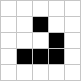
\includegraphics{figs/glider.png}
\caption{A ``Glider'' in the Game of Life.}
\label{fig:glider}
\end{center}
\end{figure}

\index{neighbor}

The game proceeds in time steps, during which each cell interacts with its neighbors in the eight adjacent cells.
At each time step, the following rules are applied:

\begin{itemize}
\small
\item A live cell with fewer than two live neighbors dies, as if by underpopulation.
\item A live cell with more than three live neighbors dies, as if by overpopulation.
\item A dead cell with exactly three live neighbors becomes a live cell, as if by reproduction.
\end{itemize}

\index{stable configuration}

Notice some consequences of these rules.
If you start with a single live cell, it dies.
If all cells are dead, no cells come to life.
But if you have four cells in a square, they keep each other alive, so that's a ``stable'' configuration.

Another initial configuration is shown in Figure~\ref{fig:blinker}.
If you start with three horizontal cells, the center cell lives, the left and right cells die, and the top and bottom cells come to life.
The result after the first time step is three vertical cells.

During the next time step, the center cell lives, the top and bottom cells die, and the left and right cells come to life.
The result is three horizontal cells, so we're back where we started, and the cycle repeats forever.

\begin{figure}[!ht]
\begin{center}
%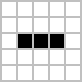
\includegraphics{figs/blinker-0.png}
%\raisebox{38pt}{~$\longrightarrow$~}
%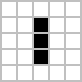
\includegraphics{figs/blinker-1.png}
%\raisebox{38pt}{~$\longrightarrow$~}
%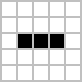
\includegraphics{figs/blinker-0.png}
%\raisebox{38pt}{~$\longrightarrow$~ \ldots}
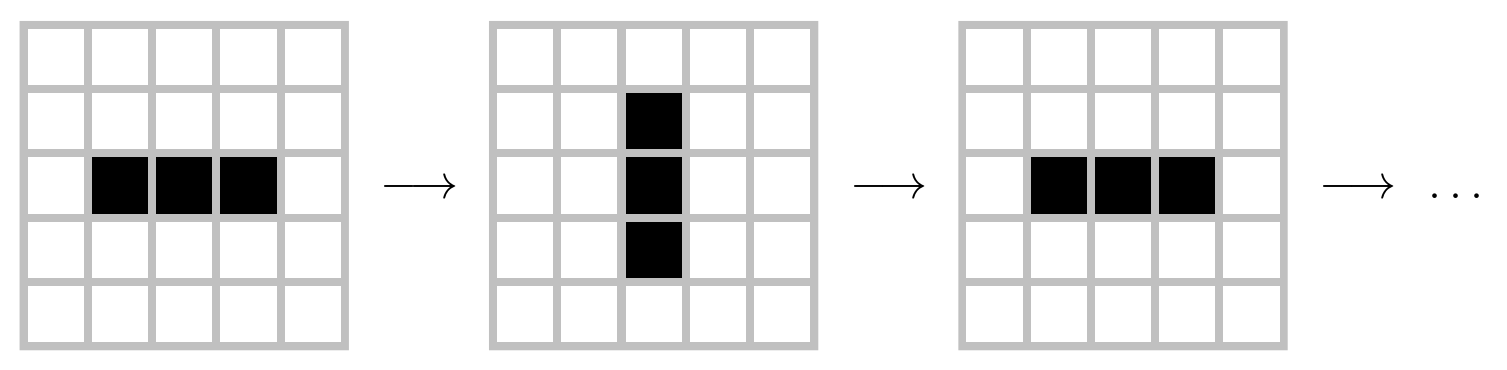
\includegraphics[trim=0 20 0 20,clip,width=0.95\linewidth]{figs/figure15-2.png}
\caption{A ``Blinker'' in the Game of Life.}
\label{fig:blinker}
\end{center}
\end{figure}

Patterns like this are called ``periodic'', because they repeat after a period of two or more time steps.
But they are also considered stable, because the total number of live cells doesn't grow over time.

Most simple starting configurations either die out quickly or reach a stable configuration.
But there are a few starting conditions that display remarkable complexity.
One of those is the R-pentomino (\url{https://www.conwaylife.com/wiki/R-pentomino}), which starts with only five cells, runs for 1,103 time steps, and ends in a stable configuration with 116 live cells.

In the following sections, we'll implement the Game of Life in Java.
We'll first implement the cells, then the grid of cells, and finally the game itself.


\section{The Cell Class}

When drawing a cell, we'll need to know its location on the screen and size in pixels.
To represent the location, we use the \java{x} and \java{y} coordinates of the upper-left corner.
And to represent the size, we use an integer, \java{size}.

\index{state}

To represent the state of a cell, we use an integer, \java{state}, which is \java{0} for dead cells and \java{1} for live cells.
We could use a \java{boolean} instead, but it's good practice to design classes to be reusable (e.g., for other games that have more states).

Here is a \java{Cell} class that declares these instance variables:

\begin{code}
public class Cell {
    private final int x;
    private final int y;
    private final int size;
    private int state;
}
\end{code}

Notice that \java{x}, \java{y}, and \java{size} are constants.
Once the cell is created, we don't want it to move or change size.
But \java{state} can and should change, so it is not a constant.

The next step is to write a constructor.
Here's one that takes \java{x}, \java{y}, and \java{size} as parameters, and sets {\tt state} to a default value:

\begin{code}
public Cell(int x, int y, int size) {
    this.x = x;
    this.y = y;
    this.size = size;
    this.state = 0;
}
\end{code}

%The following line uses the constructor to create a \java{Cell}.
%Its upper-left corner is at (0, 0), and the cell is \mbox{10 x 10} pixels.
%
%\begin{code}
%Cell cell = new Cell(0, 0, 10);
%\end{code}

The following method draws a cell.
Like the \java{paint} method in Appendix~\ref{graphics}, it takes a graphics context as a parameter:

\begin{code}
public static final Color[] COLORS = {Color.WHITE, Color.BLACK};

public void draw(Graphics g) {
    g.setColor(COLORS[state]);
    g.fillRect(x + 1, y + 1, size - 1, size - 1);
    g.setColor(Color.LIGHT_GRAY);
    g.drawRect(x, y, size, size);
}
\end{code}

The \java{draw} method uses the state of the cell to select a color from an array of \java{Color} objects.
Then it uses to \java{fillRect} to draw the center of the cell and \java{drawRect} to draw a light-gray border.

We also need methods to get and set the cell's state.
We could just provide \java{getState} and \java{setState}, but the code will be more readable if we provide methods customized for the Game of Life:

\begin{code}
public boolean isOff() {
    return state == 0;
}

public boolean isOn() {
    return state == 1;
}

public void turnOff() {
    state = 0;
}

public void turnOn() {
    state = 1;
}
\end{code}

%\java{isOff} and \java{isOn} check the state of the cell.
%\java{turnOff} and \java{turnOn} modify the state of the cell.


\section{Two-Dimensional Arrays}

\index{multidimensional array}

To represent a grid of cells, we can use a {\bf multidimensional array}.
To create a 2D array, we specify the number of rows and columns:

\begin{code}
int rows = 4;
int cols = 3;
Cell[][] array = new Cell[rows][cols];
\end{code}

The result is an array with four rows and three columns.
Initially, the elements of the array are \java{null}.
We can fill the array with \java{Cell} objects like this:

\begin{code}
for (int r = 0; r < rows; r++) {
    int y = r * size;
    for (int c = 0; c < cols; c++) {
        int x = c * size;
        array[r][c] = new Cell(x, y, size);
    }
}
\end{code}

The loop variables \java{r} and \java{c} are the row and column indexes of the cells.
The variables \java{x} and \java{y} are the coordinates, respectively.
For example, if \java{size} is 10 pixels, the cell at index (1, 2) would be at coordinates (10, 20) on the screen.

In Java, a 2D array is really an array of arrays.
You can think of it as an array of rows, where each row is an array.
Figure~\ref{fig:2D-array} shows what it looks like.

\begin{figure}[!ht]
\begin{center}
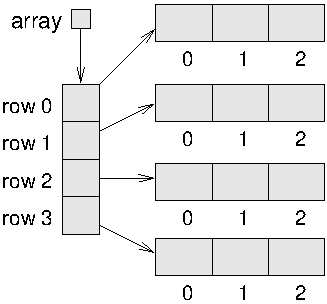
\includegraphics{figs/2D-array.pdf}
\caption{Storing rows and columns with a 2D array.}
\label{fig:2D-array}
\end{center}
\end{figure}

\index{row-major order}

%\java{array} is an array of references that refer to arrays of \java{Cell} objects.
When we write \java{array[r][c]}, Java uses the first index to select a row and the second index to select an element from the row.
This way of representing 2D data is known as {\bf row-major order}.


\section{The GridCanvas Class}

Now that we have a \java{Cell} class and a way to represent a 2D array of cells, we can write a class to represent a grid of cells.
We encapsulate the code from the previous section and generalize it to construct a grid with any number of rows and columns:

\begin{code}
public class GridCanvas extends Canvas {
    private Cell[][] array;

    public GridCanvas(int rows, int cols, int size) {
        array = new Cell[rows][cols];
        for (int r = 0; r < rows; r++) {
            int y = r * size;
            for (int c = 0; c < cols; c++) {
                int x = c * size;
                array[r][c] = new Cell(x, y, size);
            }
        }

        // set the canvas size
        setSize(cols * size, rows * size);
    }
}
\end{code}

\index{IS-A}
\index{HAS-A}
\index{Graphics}

Using vocabulary from the previous chapter, \java{GridCanvas} ``is~a'' \java{Canvas} that ``has~a'' 2D array of cells.
By extending the \java{Canvas} class from \java{java.awt}, we inherit methods for drawing graphics on the screen.

\index{nested!arrays}
\index{traversal}

In fact, the code is surprisingly straightforward: to draw the grid, we simply draw each cell.
We use nested \java{for} loops to traverse the 2D array:

\begin{code}
public void draw(Graphics g) {
    for (Cell[] row : array) {
        for (Cell cell : row) {
            cell.draw(g);
        }
    }
}
\end{code}

The outer loop traverses the rows; the inner loop traverses the cells in each row.
You can almost read this method in English: ``For each \java{row} in the \java{array}, and for each \java{cell} in the \java{row}, draw the \java{cell} in the graphics context.''
Each cell contains its coordinates and size, so it knows how to draw itself.

Classes that extend \java{Canvas} are supposed to provide a method called \java{paint} that ``paints'' the contents of the \java{Canvas}.
It gets invoked when the \java{Canvas} is created and anytime it needs to be redrawn; for example, when its window is moved or resized.

Here's the \java{paint} method for \java{GridCanvas}.
When the window management system calls \java{paint}, \java{paint} calls \java{draw}, which draws the cells:

\begin{code}
public void paint(Graphics g) {
    draw(g);
}
\end{code}


\section{Other Grid Methods}

In addition to \java{draw} and \java{paint}, the \java{GridCanvas} class provides methods for working with the grid itself.
\java{numRows} and \java{numCols} return the number of rows and columns.
We can get this information from the 2D array, using \java{length}:

\begin{code}
public int numRows() {
    return array.length;
}

public int numCols() {
    return array[0].length;
}
\end{code}

Because we are using row-major order, the 2D array is an array of rows.
\java{numRows} simply returns the length of the rows array.
\java{numCols} returns the length of the first row, which is the number of columns.
Since the rows all have the same length, we have to check only one.

\java{GridCanvas} also provides a method that gets the \java{Cell} at a given location, and for convenience when starting the game, a method that turns on the \java{Cell} at a given location.

\begin{code}
public Cell getCell(int r, int c) {
    return array[r][c];
}

public void turnOn(int r, int c) {
    array[r][c].turnOn();
}
\end{code}


\section{Starting the Game}
\label{conwaymain}

Now we're ready to implement the game.
To encapsulate the rules of GoL, we define a class named \java{Conway}.
The \java{Conway} class ``has~a'' \java{GridCanvas} that represents the state of the game.

This constructor makes a \java{GridCanvas} with 5 rows and 10 columns, with cells that are 20 pixels wide and high.
It then sets up the initial conditions:

\begin{code}
public class Conway {
    private GridCanvas grid;

    public Conway() {
        grid = new GridCanvas(5, 10, 20);
        grid.turnOn(2, 1);
        grid.turnOn(2, 2);
        grid.turnOn(2, 3);
        grid.turnOn(1, 7);
        grid.turnOn(2, 7);
        grid.turnOn(3, 7);
    }
}
\end{code}

Before we implement the rest of the game, we'll write a \java{main} method that creates a \java{Conway} object and displays it.
We can use this method to test \java{Cell} and \java{GridCanvas}, and to develop the other methods we need:

\begin{code}
public static void main(String[] args) {
    String title = "Conway's Game of Life";
    Conway game = new Conway();
    JFrame frame = new JFrame(title);
    frame.setDefaultCloseOperation(JFrame.EXIT_ON_CLOSE);
    frame.setResizable(false);
    frame.add(game.grid);
    frame.pack();
    frame.setVisible(true);
    game.mainloop();
}
\end{code}

\index{JFrame}

After constructing the \java{game} object, \java{main} constructs a \java{JFrame}, which creates a window on the screen.
The \java{JFrame} is configured\footnotemark{} to exit the program when closed.
Resizing the window is disabled.

\footnotetext{
We are using \java{JFrame} (in \java{javax.swing}) instead of \java{Frame} (in \java{java.awt}) for simplicity.
\java{Frame} does not provide a default close operation; it requires you to implement a method to be called when the user closes the window.
}

\java{main} then adds the \java{GridCanvas} inside the frame, resizes (``packs'') the frame to fit the canvas, and makes the frame visible.
Figure~\ref{fig:conway} shows the result.

\begin{figure}[!ht]
\begin{center}
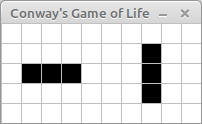
\includegraphics{figs/conway.png}
\caption{Screenshot of the initial \java{Conway} application.}
\label{fig:conway}
\end{center}
\end{figure}


\section{The Simulation Loop}
\label{mainloop}

At the end of \java{main}, we call \java{mainloop}, which uses a \java{while} loop to simulate the time steps of the Game of Life.
Here's a rough draft of this method:

\begin{code}
private void mainloop() {
    while (true) {
        this.update();
        grid.repaint();
        Thread.sleep(500);    // compiler error
    }
}
\end{code}

During each time step, we update the state of the game and repaint the \java{grid}.
We will present the \java{update} method in Section~\ref{sec:update}.

\java{repaint} comes from the \java{Canvas} class.
By default, it calls the \java{paint} method we provided, which calls \java{draw}.
The reason we use it here is that \java{repaint} does not require a \java{Graphics} object as a parameter.

\index{Thread.sleep}
\index{sleep}

\java{Thread.sleep(500)} causes the program to ``sleep'' for 500 milliseconds, or a half second.
Otherwise, the program would run so fast we would not be able to see the animation.

\index{InterruptedException}
\index{exception!Interrupted}

There's just one problem: compiling this code results in the error ``unreported exception InterruptedException''.
This message means we need to do some exception handling.


\section{Exception Handling}

So far, the only exceptions you have seen are run-time errors like ``array index out of bounds'' and ``null pointer''.
When one of these exceptions occurs, Java displays a message and ends the program.

If you don't want the program to end, you can handle exceptions with a \java{try}-\java{catch} statement.
The syntax is similar to an \java{if}-\java{else} statement, and the logic is, too.
Here's what it looks like:

\index{try}
\index{catch}
\index{statement!try}
\index{statement!catch}

\begin{code}
try {
    Thread.sleep(500);
} catch (InterruptedException e) {
    // do nothing
}
\end{code}

First, Java runs the code in the try block, which calls \java{Thread.sleep} in this example.
If an \java{InterruptedException} occurs during the try block, Java executes the catch block.
In this example, the catch block contains a comment, so it doesn't do anything.

If a different exception occurs during the try block, Java does whatever it would do otherwise, which is probably to display a message and end the program.
If no exceptions occur during the try block, the catch block doesn't run and the program continues.

In this example, the effect of the \java{try}-\java{catch} statement is to ignore an ``interrupted'' exception if it occurs.
As an alternative, we could use the catch block to display a customized message, end the program, or handle the exception in whatever way is appropriate.
For example, if user input causes an exception, we could catch the exception and prompt the user to try again later.

There's more to learn about exception handling.
You can read about exceptions in the Java tutorials (see \url{https://thinkjava.org/exceptions}).


\section{Counting Neighbors}

\index{neighbor}

Now that you know about \java{try} and \java{catch}, we can use them to implement a useful method in \java{GridCanvas}.
Part of the GoL logic is to count the number of live neighbors.
Most cells have eight neighbors, as shown in Figure~\ref{fig:neighbors}.

However, cells on the edges and in the corners have fewer neighbors.
If we try to count all possible neighbors, we'll go out of bounds.
%(Normally in the Game of Life, we don't have this problem because the grid size is infinite.
%But we thought that version might be a bit much for this chapter!)
The following method uses a \java{try}-\java{catch} statement to deal with these special cases:

\begin{code}
public int test(int r, int c) {
    try {
        if (array[r][c].isOn()) {
            return 1;
        }
    } catch (ArrayIndexOutOfBoundsException e) {
        // cell doesn't exist
    }
    return 0;
}
\end{code}

\begin{figure}[!ht]
\begin{center}
%\begin{tabular}{|p{1em}|p{1em}|p{1em}|p{1em}|p{1em}|}
%\hline
%  &   &   &   &   \\
%\hline
%  & 1 & 2 & 3 &   \\
%\hline
%  & 4 & * & 5 &   \\
%\hline
%  & 6 & 7 & 8 &   \\
%\hline
%  &   &   &   &   \\
%\hline
%\end{tabular}
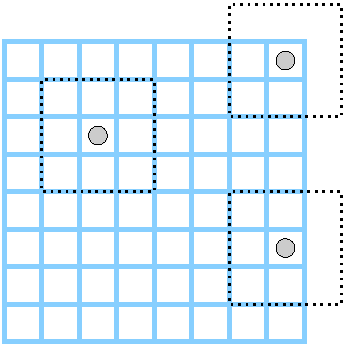
\includegraphics[height=140pt]{figs/grid.pdf}
\caption{Cells in the interior of the grid have eight neighbors.
Cells in the corners and along the edges have fewer neighbors.}
\label{fig:neighbors}
\end{center}
\end{figure}

The \java{test} method takes a row index, \java{r}, and a column index, \java{c}.
It tries to look up the \java{Cell} at that location.
If both indexes are in bounds, the \java{Cell} exists.
In that case, \java{test} returns \java{1} if the \java{Cell} is on.
Otherwise, it skips the catch block and returns \java{0}.

If either index is out of bounds, the array lookup throws an exception, but the catch block ignores it.
Then \java{test} resumes and returns \java{0}.
So the non-existent cells around the perimeter are considered to be off.

Now we can use \java{test} to implement \java{countAlive}, which takes a grid location, \java{(r, c)}, and returns the number of live neighbors surrounding that location:

\begin{code}
private int countAlive(int r, int c) {
    int count = 0;
    count += grid.test(r - 1, c - 1);
    count += grid.test(r - 1, c);
    count += grid.test(r - 1, c + 1);
    count += grid.test(r, c - 1);
    count += grid.test(r, c + 1);
    count += grid.test(r + 1, c - 1);
    count += grid.test(r + 1, c);
    count += grid.test(r + 1, c + 1);
    return count;
}
\end{code}

Because \java{test} handles ``out of bounds'' exceptions, \java{countAlive} works for any values of \java{r} and \java{c}.


\section{Updating the Grid}
\label{sec:update}

Now we are ready to write \java{update}, which gets invoked each time through the simulation loop.
It uses the GoL rules to compute the state of the grid after the next time step:

\begin{code}
public void update() {
    int[][] counts = countNeighbors();
    updateGrid(counts);
}
\end{code}

The rules of GoL specify that you have to update the cells ``simultaneously''; that is, you have to count the neighbors for all cells before you can update any of them.

We do that by traversing the grid twice: first, \java{countNeighbors} counts the live neighbors for each cell and puts the results in an array named \java{counts}; second, \java{updateGrid} updates the cells.
Here's \java{countNeighbors}:

\begin{code}
private int[][] countNeighbors() {
    int rows = grid.numRows();
    int cols = grid.numCols();

    int[][] counts = new int[rows][cols];
    for (int r = 0; r < rows; r++) {
        for (int c = 0; c < cols; c++) {
            counts[r][c] = countAlive(r, c);
        }
    }
    return counts;
}
\end{code}

\java{countNeighbors} traverses the cells in the grid and uses \java{countAlive} from the previous section to count the neighbors.
The return value is a 2D array of integers with the same size as \java{grid}.
Figure~\ref{fig:countNeigh} illustrates an example.

\begin{figure}[!ht]
\begin{center}
%\begin{minipage}{160pt}
%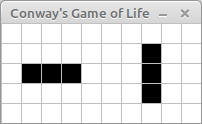
\includegraphics[trim=0 0 0 23pt,clip,width=150pt]{figs/conway.png}
%\end{minipage}
%\begin{minipage}{200pt}
%\begin{verbatim}
%{{0, 0, 0, 0, 0, 0, 1, 1, 1, 0},
% {1, 2, 3, 2, 1, 0, 2, 1, 2, 0},
% {1, 1, 2, 1, 1, 0, 3, 2, 3, 0},
% {1, 2, 3, 2, 1, 0, 2, 1, 2, 0},
% {0, 0, 0, 0, 0, 0, 1, 1, 1, 0}}
%\end{verbatim}
%\end{minipage}
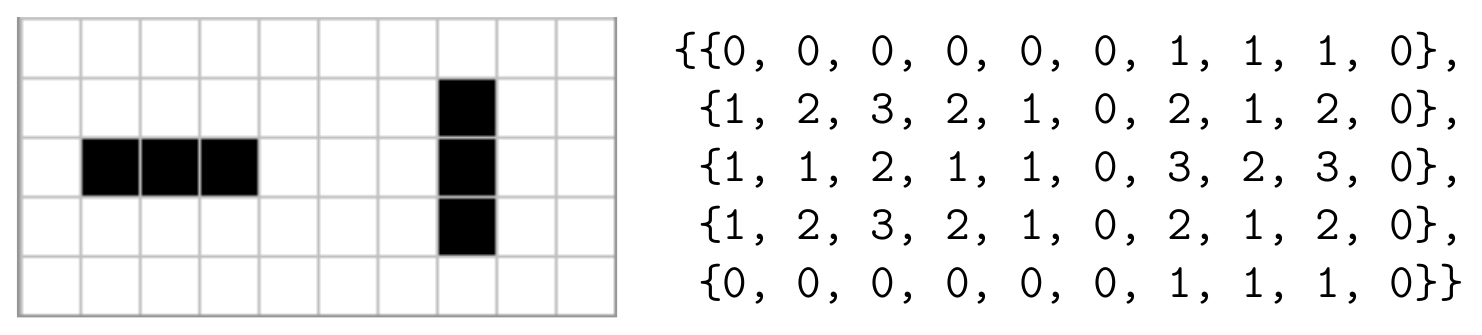
\includegraphics[trim=0 15 0 15,clip,width=0.93\linewidth]{figs/figure15-6.png}
\caption{The result of \java{countNeighbors} for the grid in Section~\ref{conwaymain}.}
\label{fig:countNeigh}
\end{center}
\end{figure}

In contrast to the \java{draw} method of \java{GridCanvas}, which uses enhanced \java{for} loops, \java{countNeighbors} uses standard \java{for} loops.
The reason is that, in this example, we need the indexes \java{r} and \java{c} to store the neighbor counts.

\java{updateGrid} uses \java{getCell} to select each \java{Cell} in the grid, and \java{updateCell} to do the update:

\begin{code}
private void updateGrid(int[][] counts) {
    int rows = grid.numRows();
    int cols = grid.numCols();

    for (int r = 0; r < rows; r++) {
        for (int c = 0; c < cols; c++) {
            Cell cell = grid.getCell(r, c);
            updateCell(cell, counts[r][c]);
        }
    }
}
\end{code}

\java{updateCell} implements the GoL rules: if the cell is alive, it dies if it has fewer than two or more than three neighbors; if the cell is dead, it comes to life if it has exactly three:

\begin{code}
private static void updateCell(Cell cell, int count) {
    if (cell.isOn()) {
        if (count < 2 || count > 3) {
            cell.turnOff();
        }
    } else {
        if (count == 3) {
            cell.turnOn();
        }
    }
}
\end{code}

Notice that \java{updateGrid} and \java{updateCell} are both \java{private}, because they are helper methods not intended to be invoked from outside the class.
\java{updateCell} is also \java{static}, because it does not depend on \java{grid}.

Now our implementation of the Game of Life is complete.
We think it's is pretty fun, and we hope you agree.
But more importantly, this example is meant to demonstrate the use of 2D arrays and an object-oriented design that's a little more substantial than in previous chapters.

%In the exercises at the end of this chapter, you'll have a chance to run the code, test other initial conditions, and explore other games with similar rules.


\section{Vocabulary}

\begin{description}

\term{multidimensional array}
An array with more than one dimension; a 2D array is an ``array of arrays''.

\term{row-major order}
Storing data in a 2D array, first by rows and then by columns.

\end{description}


\section{Exercises}

The code for this chapter is in the {\it ch15} directory of {\it ThinkJavaCode2}.
See page~\pageref{code} for instructions on how to download the repository.
Before you start the exercises, we recommend that you compile and run the examples.


\begin{exercise}
In \java{GridCanvas}, write a method named \java{countOn} that returns the total number of cells that are ``on''.
This method can be used, for example, to track the population in Game of Life over time.
\end{exercise}


\begin{exercise}
In our version of the Game of Life, the grid has a finite size.
As a result, moving objects such as Gliders either crash into the wall or go out of bounds.

An interesting variation of the Game of Life is a ``toroidal'' grid, meaning that the cells ``wrap around'' on the edges.
Modify the \java{test} method of \java{GridCanvas} so that the coordinates \java{r} and \java{c} map to the opposite side of the grid if they are too low or two high.

Run your code with a Glider (see Figure~\ref{fig:glider}) to see if it works.
You can initialize the Glider by modifying the constructor in the \java{Conway} class, or by reading it from a file (see the next exercise).
\end{exercise}


%CSM idea for another exercise: 2D arrays -- grow/shrink the grid
%ABD: Good idea, but I think we have enough for now.

%\begin{exercise}
%Another way to handle edge collisions is to expand the grid as needed.
%\end{exercise}


\begin{exercise}

The LifeWiki site (\url{https://conwaylife.com/wiki/}) has a fascinating collection of patterns for the Game of Life.
These patterns are stored in a file format that is easy to read, in files with the suffix ``.cells''.

For example, here is an \mbox{8 x 10} grid with a Glider near the upper-left corner:

\begin{stdout}
!Name: Glider
..........
..O.......
...O......
.OOO......
..........
..........
..........
..........
\end{stdout}

Lines that begin with \java{!} are comments and should be ignored.
The rest of the file describes the grid, row by row.
A period represents a dead cell, and an uppercase {\tt O} represents a live cell.
See \url{https://conwaylife.com/wiki/Plaintext} for more examples.

\begin{enumerate}

\item Create a plain text file with the contents shown above, and save the file as {\it glider.cells} in the same directory as your code.

% ABD: Should this be a constructor?  I would make it a static method that builds and returns a Conway object, on the principle that constructors generally take parameters that line up with the instance variables, and methods that do substantial work should not be constructors.  But that might be a Pythonic principle that isn't Java-idiomatic.

\item Define a constructor for the \java{Conway} class that takes a string representing the name (or path) of a ``.cells'' file.
Here is a starting point:

\begin{code}
public Conway(String path) {
    File file = new File(path);
    Scanner scan = new Scanner(file);
}
\end{code}

\item Modify the \java{main} method to invoke the constructor as follows:

\begin{code}
Conway game = new Conway("glider.cells");
\end{code}

\item Handle the \java{FileNotFoundException} that may be thrown when creating a \java{Scanner} for a \java{File} by invoking \java{printStackTrace} on the exception object and calling \java{System.exit()} with a status of \java{1}, indicating an error.

\item Continue implementing the constructor by reading all non-comment lines into an \java{ArrayList} via \java{hasNextLine} and \java{nextLine} of the \java{Scanner}.

\item Determine the number of rows and columns of the grid by examining the \java{ArrayList} contents.

\item Create and initialize a \java{GridCanvas} based on the \java{ArrayList}.

\end{enumerate}

Once your constructor is working, you will be able to run many of the patterns on the LifeWiki.
You might want to add a margin of empty cells around the initial pattern, to give it room to grow.

\end{exercise}


\begin{exercise}
Some files on the LifeWiki use ``run-length encoding'' (RLE) instead of plain text.
The basic idea of RLE is to describe the number of dead and alive cells, rather than type out each individual cell.

For example, {\it glider.cells} from the previous exercise could be represented this way with RLE:

\begin{stdout}
#C Name: Glider
x = 10, y = 8
$2bo$3bo$b3o!
\end{stdout}%$

The first line specifies \verb|x| (the number of columns) and \verb|y| (the number of rows).
Subsequent lines consist of the letters \verb|b| (dead), \verb|o| (alive), and \verb|$| (end of line), optionally preceded by a count.
The pattern ends with \verb|!|, after which any remaining file contents are ignored.

Lines beginning with \verb|#| have special meaning and are not part of the pattern.
For example, \verb|#C| is a comment line.
You can read more about RLE format on \url{https://conwaylife.com/wiki/RLE}.

\begin{enumerate}

\item Create a plain text file with the preceding contents, and save the file as {\it glider.rle} in the same directory as your code.

%ABD: As in the previous exercise, should this be a constructor?  And either way, should it be a separate method, or modify the other method to read both formats?

\item Modify your constructor from the previous exercise to check the last three characters of the \java{path}.
If they are \java{"rle"}, then you will need to process the file as RLE.
Otherwise, assume the file is in ``.cells'' format.

\item In the end, your constructor should be able to read and initialize grids in both formats.
Test your constructor by modifying the \java{main} method to read different files.

\end{enumerate}

\end{exercise}
